% Options for packages loaded elsewhere
\PassOptionsToPackage{unicode}{hyperref}
\PassOptionsToPackage{hyphens}{url}
\PassOptionsToPackage{dvipsnames,svgnames,x11names}{xcolor}
%
\documentclass[
]{article}

\usepackage{amsmath,amssymb}
\usepackage{iftex}
\ifPDFTeX
  \usepackage[T1]{fontenc}
  \usepackage[utf8]{inputenc}
  \usepackage{textcomp} % provide euro and other symbols
\else % if luatex or xetex
  \usepackage{unicode-math}
  \defaultfontfeatures{Scale=MatchLowercase}
  \defaultfontfeatures[\rmfamily]{Ligatures=TeX,Scale=1}
\fi
\usepackage{lmodern}
\ifPDFTeX\else  
    % xetex/luatex font selection
\fi
% Use upquote if available, for straight quotes in verbatim environments
\IfFileExists{upquote.sty}{\usepackage{upquote}}{}
\IfFileExists{microtype.sty}{% use microtype if available
  \usepackage[]{microtype}
  \UseMicrotypeSet[protrusion]{basicmath} % disable protrusion for tt fonts
}{}
\makeatletter
\@ifundefined{KOMAClassName}{% if non-KOMA class
  \IfFileExists{parskip.sty}{%
    \usepackage{parskip}
  }{% else
    \setlength{\parindent}{0pt}
    \setlength{\parskip}{6pt plus 2pt minus 1pt}}
}{% if KOMA class
  \KOMAoptions{parskip=half}}
\makeatother
\usepackage{xcolor}
\setlength{\emergencystretch}{3em} % prevent overfull lines
\setcounter{secnumdepth}{5}
% Make \paragraph and \subparagraph free-standing
\makeatletter
\ifx\paragraph\undefined\else
  \let\oldparagraph\paragraph
  \renewcommand{\paragraph}{
    \@ifstar
      \xxxParagraphStar
      \xxxParagraphNoStar
  }
  \newcommand{\xxxParagraphStar}[1]{\oldparagraph*{#1}\mbox{}}
  \newcommand{\xxxParagraphNoStar}[1]{\oldparagraph{#1}\mbox{}}
\fi
\ifx\subparagraph\undefined\else
  \let\oldsubparagraph\subparagraph
  \renewcommand{\subparagraph}{
    \@ifstar
      \xxxSubParagraphStar
      \xxxSubParagraphNoStar
  }
  \newcommand{\xxxSubParagraphStar}[1]{\oldsubparagraph*{#1}\mbox{}}
  \newcommand{\xxxSubParagraphNoStar}[1]{\oldsubparagraph{#1}\mbox{}}
\fi
\makeatother


\providecommand{\tightlist}{%
  \setlength{\itemsep}{0pt}\setlength{\parskip}{0pt}}\usepackage{longtable,booktabs,array}
\usepackage{calc} % for calculating minipage widths
% Correct order of tables after \paragraph or \subparagraph
\usepackage{etoolbox}
\makeatletter
\patchcmd\longtable{\par}{\if@noskipsec\mbox{}\fi\par}{}{}
\makeatother
% Allow footnotes in longtable head/foot
\IfFileExists{footnotehyper.sty}{\usepackage{footnotehyper}}{\usepackage{footnote}}
\makesavenoteenv{longtable}
\usepackage{graphicx}
\makeatletter
\newsavebox\pandoc@box
\newcommand*\pandocbounded[1]{% scales image to fit in text height/width
  \sbox\pandoc@box{#1}%
  \Gscale@div\@tempa{\textheight}{\dimexpr\ht\pandoc@box+\dp\pandoc@box\relax}%
  \Gscale@div\@tempb{\linewidth}{\wd\pandoc@box}%
  \ifdim\@tempb\p@<\@tempa\p@\let\@tempa\@tempb\fi% select the smaller of both
  \ifdim\@tempa\p@<\p@\scalebox{\@tempa}{\usebox\pandoc@box}%
  \else\usebox{\pandoc@box}%
  \fi%
}
% Set default figure placement to htbp
\def\fps@figure{htbp}
\makeatother

\usepackage{booktabs}
\usepackage{longtable}
\usepackage{array}
\usepackage{multirow}
\usepackage{wrapfig}
\usepackage{float}
\usepackage{colortbl}
\usepackage{pdflscape}
\usepackage{tabu}
\usepackage{threeparttable}
\usepackage{threeparttablex}
\usepackage[normalem]{ulem}
\usepackage{makecell}
\usepackage{xcolor}
\makeatletter
\@ifpackageloaded{caption}{}{\usepackage{caption}}
\AtBeginDocument{%
\ifdefined\contentsname
  \renewcommand*\contentsname{Indholdsfortegnelse}
\else
  \newcommand\contentsname{Indholdsfortegnelse}
\fi
\ifdefined\listfigurename
  \renewcommand*\listfigurename{Figuroversigt}
\else
  \newcommand\listfigurename{Figuroversigt}
\fi
\ifdefined\listtablename
  \renewcommand*\listtablename{Tabeloversigt}
\else
  \newcommand\listtablename{Tabeloversigt}
\fi
\ifdefined\figurename
  \renewcommand*\figurename{Figur}
\else
  \newcommand\figurename{Figur}
\fi
\ifdefined\tablename
  \renewcommand*\tablename{Tabel}
\else
  \newcommand\tablename{Tabel}
\fi
}
\@ifpackageloaded{float}{}{\usepackage{float}}
\floatstyle{ruled}
\@ifundefined{c@chapter}{\newfloat{codelisting}{h}{lop}}{\newfloat{codelisting}{h}{lop}[chapter]}
\floatname{codelisting}{Liste}
\newcommand*\listoflistings{\listof{codelisting}{Listeoversigt}}
\makeatother
\makeatletter
\makeatother
\makeatletter
\@ifpackageloaded{caption}{}{\usepackage{caption}}
\@ifpackageloaded{subcaption}{}{\usepackage{subcaption}}
\makeatother

\ifLuaTeX
\usepackage[bidi=basic]{babel}
\else
\usepackage[bidi=default]{babel}
\fi
\babelprovide[main,import]{danish}
% get rid of language-specific shorthands (see #6817):
\let\LanguageShortHands\languageshorthands
\def\languageshorthands#1{}
\usepackage{bookmark}

\IfFileExists{xurl.sty}{\usepackage{xurl}}{} % add URL line breaks if available
\urlstyle{same} % disable monospaced font for URLs
\hypersetup{
  pdftitle={Arbejdsløshed - Ugeeksamen i Forecasting},
  pdfauthor={Christine Hegelund; Jing Wei; Marcus Nielsen},
  pdflang={da},
  colorlinks=true,
  linkcolor={blue},
  filecolor={Maroon},
  citecolor={Blue},
  urlcolor={Blue},
  pdfcreator={LaTeX via pandoc}}


\title{Arbejdsløshed - Ugeeksamen i Forecasting}
\author{Christine Hegelund \and Jing Wei \and Marcus Nielsen}
\date{2025-06-13}

\begin{document}
\maketitle


\maketitle
\thispagestyle{empty}
\begin{center}
\large{Forecasting Eksamen} \\[3em]
\end{center}
\begin{center}
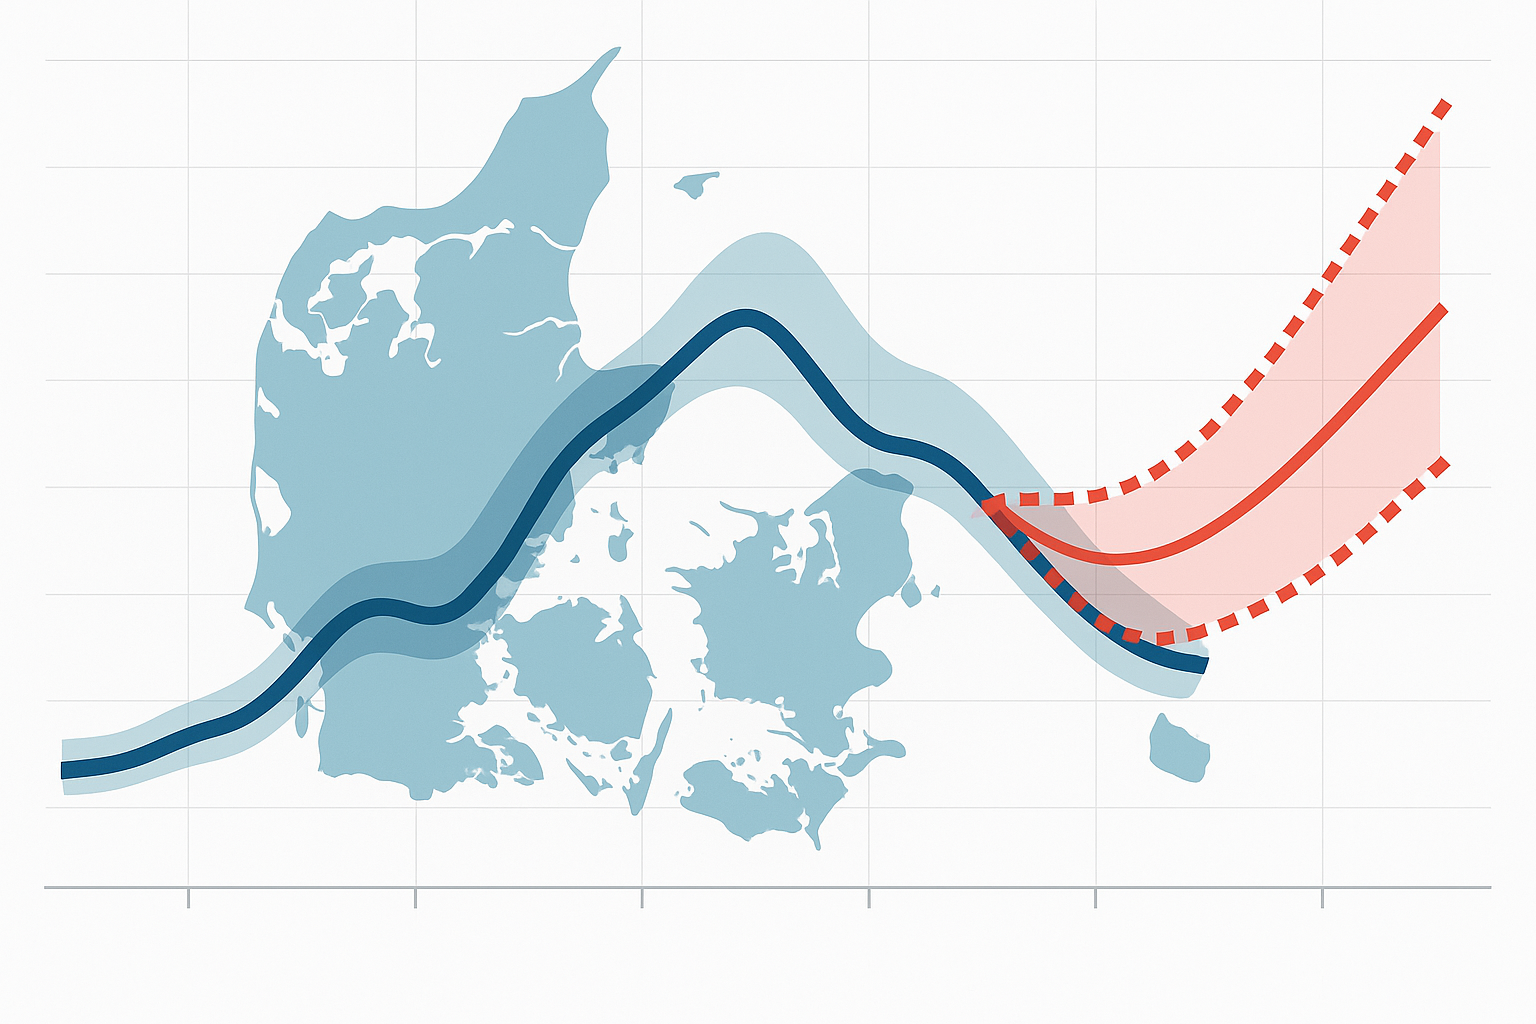
\includegraphics[width=0.9\textwidth]{fotos/forside.png} \\[2em]
\end{center}
\begin{center}
\fcolorbox{gray}{white}{
\parbox{0.8\textwidth}{
\centering
\textbf{Antal tegn (inkl. mellemrum): 97023}
}}
\end{center}
\begin{center}
\textbf{Vejledere:} \\
Bjarne Taulo Sørensen \\
\end{center}

\newpage

\addtocontents{toc}{\protect\setcounter{tocdepth}{-1}}

\section*{Tabel over figurer}\label{tabel-over-figurer}
\addcontentsline{toc}{section}{Tabel over figurer}

\thispagestyle{empty}

\newpage

\pagenumbering{arabic}
\setcounter{page}{1}
\tableofcontents
\newpage

\section{Introduktion}\label{introduktion}

Formålet med denne analyse er at modellere og forudsige
arbejdsløshedstal i Danmark opdelt på region og køn, baseret på
månedlige data fra 2007 til 2019. Ved hjælp af klassiske
tidsseriemodeller, herunder ARIMA, ETS og en simpel benchmarkmodel,
analyseres trends, sæsonvariation og residualer i data.

Opgaven er struktureret omkring faserne i en klassisk tidsserieanalyse:
fra eksplorativ dataanalyse og dekomposition til modelvalg,
modelvalidering via time series cross-validation og endelig forecast for
året 2020. Den bedste model vælges individuelt for hver af de ti serier
(5 regioner × 2 køn) baseret på performance-metrikker (RMSE og MAPE).

Der lægges vægt på at dokumentere og begrunde de metodiske valg, med
udgangspunkt i pensum og best practice fra faget. Prognoserne
præsenteres både numerisk og grafisk, og resultaterne sammenlignes på
tværs af serier.

Analysen er udelukkende baseret på de udleverede data.
Forretningsmæssige forklaringer og COVID-relaterede effekter er bevidst
udeladt, i henhold til opgavens afgrænsning.

\section{Problemformulering}\label{problemformulering}

Hvordan kan klassiske tidsseriemodeller anvendes til at analysere og
forudsige arbejdsløsheden i Danmark, fordelt på region og køn, baseret
på månedlige data fra 2007 til 2019?

Med udgangspunkt i metoder som ARIMA, ETS og en simpel benchmarkmodel er
formålet at:

\begin{itemize}
\tightlist
\item
  identificere trends og sæsonmønstre i arbejdsløsheden gennem
  eksplorativ dataanalyse og dekomposition
\item
  finde og validere den bedst egnede model for hver serie ved brug af
  time series cross-validation og performance-metrikker som RMSE og MAPE
\item
  forecaste arbejdsløsheden for året 2020 med kvantificeret usikkerhed
  via prædiktionsintervaller
\item
  sammenligne resultaterne på tværs af regioner og køn for at belyse
  forskelle i modelperformance og arbejdsløshedsniveauer
\end{itemize}

\subsection{Afgrænsning}\label{afgruxe6nsning}

Analysen er udelukkende baseret på de udleverede data og fokuserer på
anvendelse og vurdering af klassiske forecasting-metoder.

Der inddrages ikke eksterne faktorer som COVID-19, konjunkturændringer
eller politiske tiltag. Der gives heller ikke forretningsmæssige
anbefalinger, da formålet er metodisk -- ikke strategisk.

Fokus er således på at demonstrere korrekt og fagligt funderet
anvendelse af tidsserieanalyse og forecasting-teknikker i en
struktureret, reproducerbar analyse.

\subsubsection{Anvendelse af
AI-værktøj}\label{anvendelse-af-ai-vuxe6rktuxf8j}

I forbindelse med udarbejdelsen af denne opgave er ChatGPT (GPT-4o)
benyttet som et støtteværktøj. Værktøjet har primært været anvendt til
idéudvikling, sproglig sparring, forbedring af formuleringers klarhed,
grammatisk gennemgang samt støtte ved udformning af enkelte kodestumper.
Anvendelsen har udelukkende omfattet sproglige, strukturelle og tekniske
elementer. Alt analytisk, fortolkende og konkluderende indhold er
selvstændigt udarbejdet af gruppens medlemmer.

\subsection{Definitioner/forkortelser}\label{definitionerforkortelser}

I dette afsnit afklares centrale begreber og forkortelser, der anvendes
gennem opgaven, for at sikre en ensartet forståelse.

\subsection{Struktur}\label{struktur}

Opgaven er opbygget i overensstemmelse med en klassisk tilgang til
tidsserieanalyse. Først gennemføres en eksplorativ dataanalyse (EDA),
hvor datasættet undersøges for trend, sæsonvariation og andre
karakteristika gennem visualisering, deskriptiv statistik og
STL-dekomposition. Herefter følger modelvalgsfasen, hvor tre modeller --
ARIMA, ETS og en simpel benchmarkmodel -- estimeres for hver tidsserie.
Modellerne evalueres gennem time series cross-validation med fokus på
RMSE og MAPE, hvorefter den bedst performende model vælges for hver
serie. Afslutningsvis foretages forecast for 2020 med tilhørende
prædiktionsintervaller, efterfulgt af en sammenlignende vurdering og
konklusion.

\section{Data og forberedelse}\label{data-og-forberedelse}

Analysen er baseret på et datasæt med månedlige arbejdsløshedstal i
Danmark fra januar 2007 til december 2019. Data er opdelt på køn (mænd
og kvinder) og region (de fem danske regioner), hvilket resulterer i ti
separate tidsserier. Datasættet er udleveret i forbehandlet format som
en tsibble med korrekt angivne indeks- og nøglevariabler, hvilket gør
det velegnet til modellering i fable/tidyverts-pakken.

\section{Eksplorativ dataanalyse
(EDA)}\label{eksplorativ-dataanalyse-eda}

\subsection{Visualisering af trends og
sæsonmønstre}\label{visualisering-af-trends-og-suxe6sonmuxf8nstre}

\subsection{Deskriptive statistikker}\label{deskriptive-statistikker}

\subsection{STL-dekomposition}\label{stl-dekomposition}

\section{Modelvalg}\label{modelvalg}

\subsection{ARIMA og SARIMA}\label{arima-og-sarima}

\subsection{ETS (Exponential
Smoothing)}\label{ets-exponential-smoothing}

\subsection{Simpel benchmarkmodel}\label{simpel-benchmarkmodel}

\subsection{Kort beskrivelse af
modellerne}\label{kort-beskrivelse-af-modellerne}

\section{Modelvalidering}\label{modelvalidering}

\subsection{Time series
cross-validation}\label{time-series-cross-validation}

\subsection{Evaluering med RMSE og
MAPE}\label{evaluering-med-rmse-og-mape}

\subsection{Valg af bedste model pr.
serie}\label{valg-af-bedste-model-pr.-serie}

\subsection{Test for hvid støj}\label{test-for-hvid-stuxf8j}

\section{Forecasting}\label{forecasting}

\subsection{Træning og forecast for
2020}\label{truxe6ning-og-forecast-for-2020}

\subsection{Prædiktionsintervaller}\label{pruxe6diktionsintervaller}

\subsection{Visualisering af
forecasts}\label{visualisering-af-forecasts}

\subsection{Centrale prognoseværdier}\label{centrale-prognosevuxe6rdier}

\section{Sammenligning og
fortolkning}\label{sammenligning-og-fortolkning}

\subsection{Sammenligning på tværs af
serier}\label{sammenligning-puxe5-tvuxe6rs-af-serier}

\subsection{Tendenser mellem regioner og
køn}\label{tendenser-mellem-regioner-og-kuxf8n}

\section{Konklusion}\label{konklusion}

\newpage

\section{Kildeliste}\label{kildeliste}

\newpage

\section{Bilagsoversigt}\label{bilagsoversigt}

\begin{itemize}
\tightlist
\item
  Bilag 1: Udleverede Powerpointpræsentationer v. Michael Freundlich:
  Chefkonsulent, Erhvervsservice og facility
\end{itemize}




\end{document}
